\documentclass{beamer}
\usetheme{Hannover}
\usepackage{amsmath}
\title{EE1390 - Introduction to AI and ML}
\subtitle{Presentation}
\author{Tejas P \\ Shivam Khandelwal}
\institute{IIT Hyderabad}
\date{\today}
\begin{document}
 \begin{frame}
 \titlepage
 \end{frame}
 \section{Question}
 \begin{frame}
 \frametitle{Question 45, JEE Advanced 2015}
 If the normals of the parabola \(y^2=4x\) drawn at the end points of its latus rectum are tangents to the circle \((x-3)^2 + (y+2)^2 = r^2\), then find the value of \(r^2\).
 \end{frame}
 \begin{frame}
 \section{Solution without using matrices}
 \frametitle{Solution without using matrices}
 The end points of the latus rectum are (1,2) and (1,-2).\\Equation of normal at (1,2) is, 
 \begin{equation}
 x+y-3=0    
 \end{equation}
 \\ Equation of normal at (1,-2) is, 
  \begin{equation}
 x-y-3=0    
 \end{equation}
 Since theses normals are tangent to the circle, the perpendicular distance from centre of the circle (3,-2) to the tangent= radius. Therefore,
 \begin{equation}
 r=\frac{|3-2-3|}{\sqrt{1+1}}    
 \end{equation}
 Thus, $r^2=2$.
 \end{frame}
 \begin{frame}
 \section{Solution using matrices}
 \frametitle{Solution using matrices}
 Equation of a conic section in matrix form is,
 \begin{equation}
  \textbf{x}^T\textbf{Vx} + 2\textbf{u}^T\textbf{x}+F=0   
 \end{equation}
 Equation of the tangent at point p on the curve is,
 \begin{equation}
 (\textbf{p}^T\textbf{V}+\textbf{u}^T)\textbf{x}+\textbf{p}^T\textbf{u}+F=0    
 \end{equation}
 \\Equation of parabola \(y^2=4x\) in matrix form is, 
 \begin{equation}
     
 
 \begin{pmatrix}
 x&y
 \end{pmatrix}\begin{pmatrix}
 0&0\\
 0&1
  \end{pmatrix}\begin{pmatrix}
 x\\
 y\\

 \end{pmatrix}+\begin{pmatrix}
 -4&0
 \end{pmatrix}\begin{pmatrix}
 x\\
 y\\
 \end{pmatrix}
 = 0 \hspace{10mm}
 \end{equation}
 or,
 \begin{equation}
     
 
 \textbf{x}^T\begin{pmatrix}
 0&0\\
 0&1\\
 \end{pmatrix}\textbf{x}+\begin{pmatrix}
 -4&0\\
 \end{pmatrix}\textbf{x}=0 \hspace{10mm}        
 \end{equation}
 \end{frame}
 \begin{frame}
 Focus of parabola is at (1,0).\\\textbf{V}= \begin{pmatrix}
 0&0\\
 0&1\\
 \end{pmatrix}, \textbf{u}=\begin{pmatrix}
 -2\\
 0\\
 \end{pmatrix}, F=0.\\Equation of circle \((x-3)^2 + (y+2)^2 = r^2\) in matrix form is:\\
 \begin{equation}
     
 
 \begin{pmatrix}
 x&y\\
 \end{pmatrix} \begin{pmatrix}
 x\\
 y\\
 \end{pmatrix}
   - 2 \begin{pmatrix}
 3&-2\\
 \end{pmatrix}\begin{pmatrix}
 x\\
 y\\
 \end{pmatrix}
 =r^2 -\begin{pmatrix}
 3&-2\\
 \end{pmatrix}\begin{pmatrix}
 3\\
 -2\\
 \end{pmatrix}
 \vspace{5mm}
 
 \textbf{x}^T\textbf{x} \,-2 \begin{pmatrix}
 3&-2\\
 \end{pmatrix}\textbf{x}=r^2-13 \hspace{10mm}
 \end{equation}
  \end{frame}
  
   \begin{frame}
   
   For the circle equation,
\textbf{V}=\textbf{I}, \textbf{u}=\,\begin{pmatrix}
 -3\\
2\\
 \end{pmatrix}, F=13 - \(r^2\).


 Equation of tangent at (1,2) on parabola using formula stated above is, \\
 \begin{equation}
     
 
 \begin{pmatrix}
 1&2\\

 \end{pmatrix}\begin{pmatrix}
 0&0\\
 0&1\\
 \end{pmatrix} \textbf{x} +\begin{pmatrix}
 -2&0\\
 \end{pmatrix}\textbf{x}+\begin{pmatrix}
 1&0\\
 \end{pmatrix}\begin{pmatrix}
 -2\\
 0\\
 \end{pmatrix} = 0\\
 \vspace{5mm}
 \begin{pmatrix}
 -2&2\\
 \end{pmatrix} \textbf{x} = 2\,\,or,
 \textbf{n}^T \textbf{x}=1, where  \ \textbf{n}=\begin{pmatrix}
 -1\\
 1\\
 \end{pmatrix} \hspace{10mm}
 \end{equation}
 \\We need to find vector \textbf{m} such that \(\textbf{m}^T\textbf{n}\) = 0 in order to construct the equation of the normal. \\ 
 \vspace{5mm}
 \textbf{m}=\begin{pmatrix}
 0&1\\
 -1&0\\
 \end{pmatrix}\textbf{n}\\
 \end{frame}
 
 \begin{frame}
 \textbf{m} = 
 \begin{pmatrix}
 0&1\\
 -1&0\\
 \end{pmatrix}\begin{pmatrix}
 -1\\
1\\
 \end{pmatrix}=\begin{pmatrix}
 1\\
 1\\
 \end{pmatrix}
 
 
 \\Equation of normal at point \textbf{p} is \(\textbf{m}^T(\textbf{x}-\textbf{p})=0\)\\
 \vspace{5mm}
 Equation of normal at (1,2) is, \\\begin{pmatrix}
 2&2\\
 \end{pmatrix}(\textbf{x}-\begin{pmatrix}
 1\\
 2\\
 \end{pmatrix})=0\\
 \begin{pmatrix}
 2&2\\
 \end{pmatrix}\textbf{x} = 6\\
 Or,\\
 \begin{pmatrix}
 1&1\\
 \end{pmatrix}\textbf{x} = 3
 \end{frame}
 \begin{frame}For the circle,
 \textbf{V}=\textbf{I}, \textbf{u}=\begin{pmatrix}
 -3\\
2\\
 \end{pmatrix}, F=13 - \(r^2\).\\
 Writing the equation of tangent for circle using the general format stated above, we get, \\
 \vspace{5mm}
 (\(\textbf{p}^T\textbf{I}\)+\begin{pmatrix}
 -3&2\\
 \end{pmatrix})\textbf{x} + \(\textbf{p}^T\)\begin{pmatrix}
-3\\
2\\
 \end{pmatrix}+ 13 - \(r^2\)=0\\Comparing it with the equation of normal,\\
 \vspace{5mm}
 \textbf{p}+\begin{pmatrix}
 -3\\
 2\\
 \end{pmatrix}=\begin{pmatrix}
 1\\
 1\\
 \end{pmatrix}
 \vspace{5mm}
 \\
 \textbf{p}=\begin{pmatrix}
 4\\
 -1\\
 \end{pmatrix}
 \\Also, \(\textbf{p}^T\)\begin{pmatrix}
-3\\
2\\
 \end{pmatrix}+ 13 - \(r^2\) = -3\\
 \end{frame}
 \begin{frame}
Substituting \textbf{p} we get, 
\vspace{5mm}
\\\begin{pmatrix}
4&-1\\
 \end{pmatrix}\begin{pmatrix}
-3\\
2\\
 \end{pmatrix}+ 13 - \(r^2\) = -3\\
\vspace{5mm} 
 $-14 + 13-r^2=-3$\\
 \vspace{5mm}
 Therefore,  \(r^2\)=2
 \end{frame}
 
 \begin{frame}
     \begin{figure}

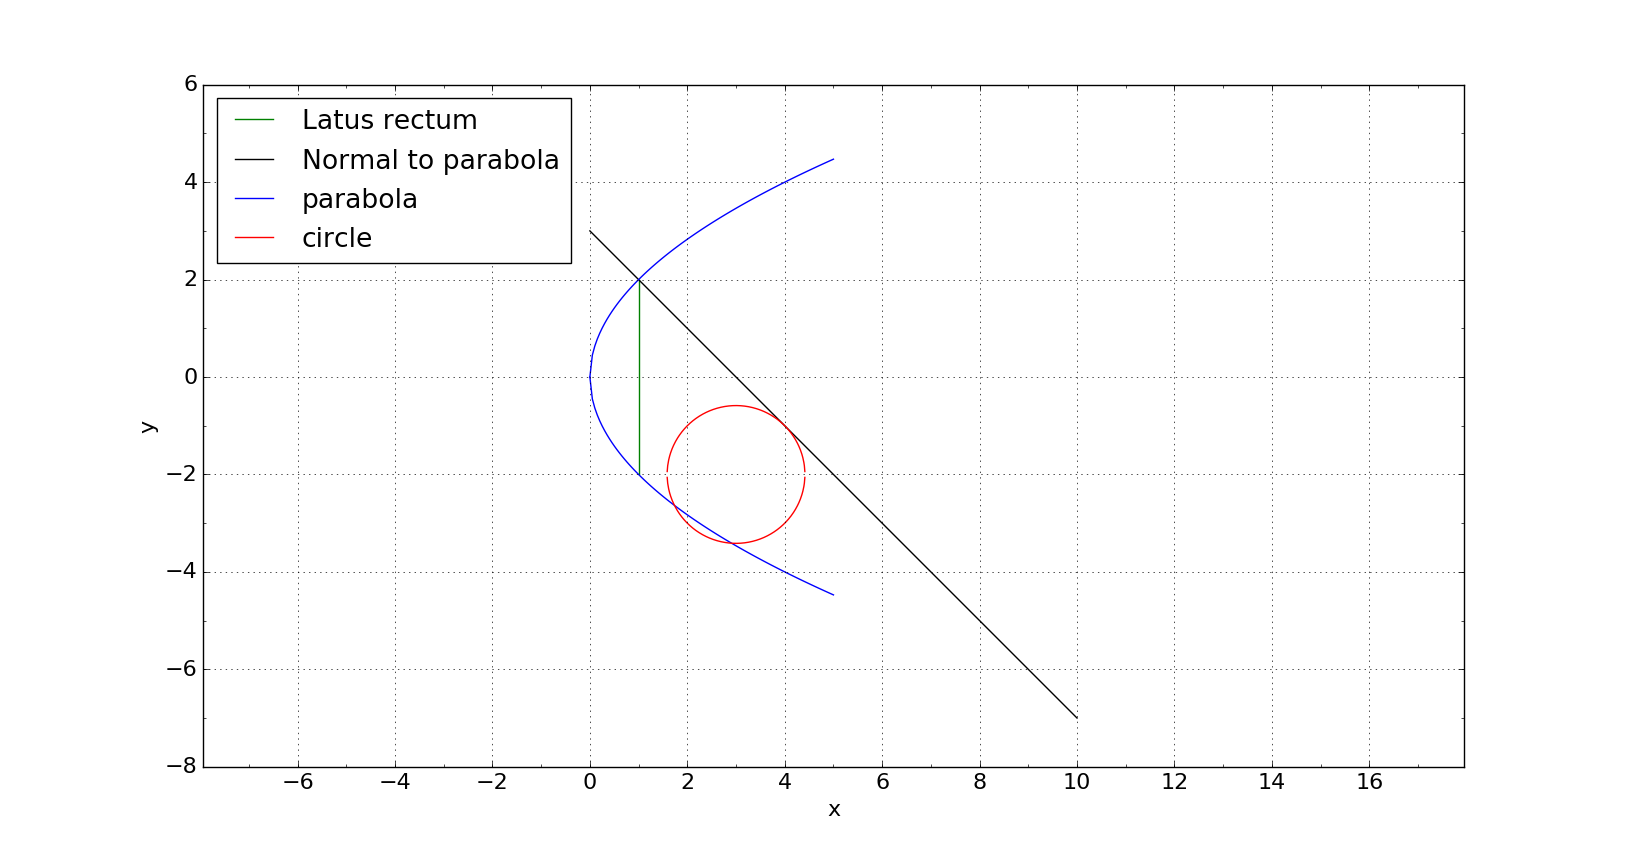
\includegraphics[scale=0.27]{fig1.png}
\caption{Graphical representation}
\end{figure}
 \end{frame}
\end{document}